% --------------------------------------------------------------------------
% Template for AASP Challenge extended abstracts; 
% to be used with: aasp.sty  - LaTeX style file, and
%          IEEEbib.bst - IEEE bibliography style file.
%
% --------------------------------------------------------------------------

\documentclass{article}
\usepackage{aasp,amsmath,graphicx,url,times,epstopdf,cite}
%\usepackage{aasp,amssymb,amsmath,graphicx,times,url}

% Example definitions.
% --------------------
\def\defeqn{\stackrel{\triangle}{=}}
\newcommand{\symvec}[1]{{\mbox{\boldmath $#1$}}}
\newcommand{\symmat}[1]{{\mbox{\boldmath $#1$}}}

% Title.
% --------------------
\title{Event Detection and Classification}

% Single addresses (uncomment and modify for single-address case).
% --------------------
\name{Sameer Chauhan, Sharang Phadke, Christian Sherland\thanks{Thanks to the Cooper Union}}
\address{Author Affiliation(s)}

% For example:
% ------------
\address{Cooper Union for the Advancement of Science and Art\\
	Electrical Engineering\\
	41 Cooper Square\\
	New York, NY 10003}

% Two addresses
% --------------------
%\twoauthors
%  {John Doe\sthanks{Thanks to ABC agency for funding.}}
%    {ABC University\\
%     500 Rainy Street,\\
%     WC1 4AB London, UK \\
%     johndoe@abc.ac.uk}
%  {Jane Doe\sthanks{Thanks to XYZ agency for funding.}}
%    {XYZ University \\
%     3040 Westfield Avenue \\
%     New Paltz, NY, USA \\
%     janedoe@xyz.edu}

\begin{document}
\ninept
\maketitle

\begin{sloppy}

\begin{abstract}
The IEEE AASP Challenge addresses the problem of acoustic event detection and classification in an office environment. Our system performs segmentation and event classification on a continuous stream of acoustic activity in an office using basic feature extraction techniques and a two layer classifier (we haven't implemented two layers yet).

\end{abstract}

\begin{keywords}
onset, offset, MFCCs, LRT
\end{keywords}

\section{Introduction}
\label{sec:intro}
The task of event detection and classification is fundamentally important in computational auditory scene analysis (CASA). Detecting events such as words in a sentence of speech, the arrival of a bus or train, or any other common occurrence in an audio stream is the first step of any speech or audio processing system that needs to make use of this information. Many such systems then need to classify the detected events in order to take appropriate actions.

In this project submission, the problem of event detection and classification, as applied to an office environment, was approached from a pattern recognition perspective. Our system consists of a segmentation stage, a feature extraction stage, and two classification stages. The first stage detects the onset and offset of events in a live recording, the second extracts features from each event that can be used to classify events, and the final stages classify each detected event
using two pre-trained classifiers. The classification system initially classifies the detected event as one of a few groups of events. The system then classifies the events in each group as a specific type of event using a set of features that extracts the most discriminatory information from the events within each group.


\section{Feature extraction}
\label{sec:feature}
In order to classify events, our system extracts a set of features from the training data. This set includes the spectral centroid, spectral flux, spectral sparsity,temporal sparsity, loudness, short time energy and Mel-frequency cepstrum coefficients (MFCC). The MFCCs are based on frequency bands equally spaced on the mel scale which approximates the human auditory system's reposnse.  
Each feature highlights different acoustic properties of the signal. Spectral sparsity is expected to be very large for pure sine tones or bells and smaller for sounds with significant ``noise'' characteristics that imply a wide frequency spectrum. Temporal sparsity is large for sounds such as footsteps in relative silence and is useful for indexing and retrieving these types of sounds. Short time energy  is analogous to the volume of the event and the spectral centroid is essentially the center of mass of the spectrum. They are both expected to be reliable indicators of silence. The spectral flux, also called spectral variation, measures how quickly the power spectrum changes. It can be used to determine the timbre of the audio signal. Different permutations of these features will be tested and the best combination will be used for the system training and classification stages of our system. 

Our feature set is computed within a 40ms window with no overlap, which forces our frames to be 40ms long. This limits our precision but increases our accuracy. In order to increase the performance of the system, we will choose features to be calculated over a long period (1s) . This 1s window will slide every 20ms and overlap will be included with the features obtained within the 40ms window to help obtain a more precise feature set for the events. 


\section{Training}
\label{sec:training}
The classification stage of our system employs two levels of classification. As input
the classifier takes in an event signal and first classifies what type of event it is.
Then based upon the type of event the signal is passed through a type-specific 
classifier which determines the exact event contained in the signal. In the second stage
each type has its own classifier.

Each level of classification in the system was trained with features extracted from the 
provided training data. The first stage classifier was trained using the full set of 
extracted features for all events. The second stage classifiers were each trained using 
features extracted only from training signals of the correct type. Additionally, the 
features used for training were chosen to best describe the type of event being classified.


\section{Segmentation}
\label{sec:segmentation}
Before events within a continuous input signal can be classified, the segments of the input which contain events must be extracted. A speech segmenter[[INSERT DUDE HERE]] accomplishes this by examining the short time energy and spectral centroid features.  The segmenter examines peaks of the features and checks them against a threshold to determine the onset and offset of events. The onset and offset times are then used to extract the portions of the input signal which contain an event and pass them on to the classification stage. 

A continuous sound file is input into the segmenter which  applies a Chebyshev Type II low pass filter. This step was added to the original segmenter to reduce the amount of background noise and increase onset and offset detection. The segmentation process requires three parameters for feature extraction: window length, step time, and the weight that will be 0 to compare the signal to a threshold. The segmenter was exhaustively tested against the development data to determine the parameters that provided optimal segmentation. Each run of the segmentation test was checked for the number of events it detected. The runs were narrowed down to those that returned the same number of events as the development data indicated. Then the mean square error was calcuated using onset and offset times and used to determine the optimal choice of parameters.$\tau_{(on)i}$ is the estimated onset time and $tau_{(off)i}$ is the estimated offset time determined by the segmenter, which is checked against the truth values $t_{on}$ and $t_{off}$.
\begin{align}
{MSE} &=\min{ (\tau_{(on)i}-t_{on} )^2 + (\tau_{(off)i}-t_{off})^2  }
\end{align}
The values for the window length, step time, and threshold weight that results in the minimum MSE were 0.05s, 0.04s and 3 respectively. During the exhaustive process, it was also determined that the threshold weight had to be an integer value. 

The segmenting function returns a two column vector where the first column indicates each onset, and the second column indicates each event offset. The signal between the onset and offset times is used in the classification stage of the system. 

\section{Classification}
\label{sec:classification}
After a set of event signals has been segmented, the classifier extracts a full set of 
features for each event signal. For each event, these features are passed into the first
level classifier. Based upon the output of the first stage classifier, each event is 
labeled with its subgroup.

Each event signal was then passed through the classifier that corresponds to its subgroup 
label and reclassified based upon the subset of features that best describes its type of
event. 

Types were chosen such that members of a given type generally have many similar features. 
The set of features that is used to determine the specific event that occurred in stage two
is the set which varies most among the members.


\section{Results}
\label{sec:results}
In order to evaluate the performance of our system we examined the percentage of frames 
correctly classified in a 5-fold cross validation, with our segmentation algorithm, and with perfect segmentation. The perfect segmentation and ground truth label for each frame were determined using the annotation to the development data.

In a noiseless environment (i.e. the 5-fold validation), the system classified events with high accuracy, as can be seen in Figure \ref{fig:kfolds}. However, given perfect segmentation on the development set, our system correctly classified 63\% of frames. This shows that, surprisingly, the input features to the classifier were significantly degraded by noise in the development set. With our segmentation algorithm, the system correctly classified only 36\% of frames. This low accuraccy demonstrates the compounding error of the detection stage.

The confusion matricies of classifier stages of the perfectly segmented events, as well as the events segmented using our algorithm can be seen in Figure \ref{fig:confmat_perfect} and Figure \ref{fig:confmat_seg} respectively.

\begin{figure}[h]
  \centering
  \centerline{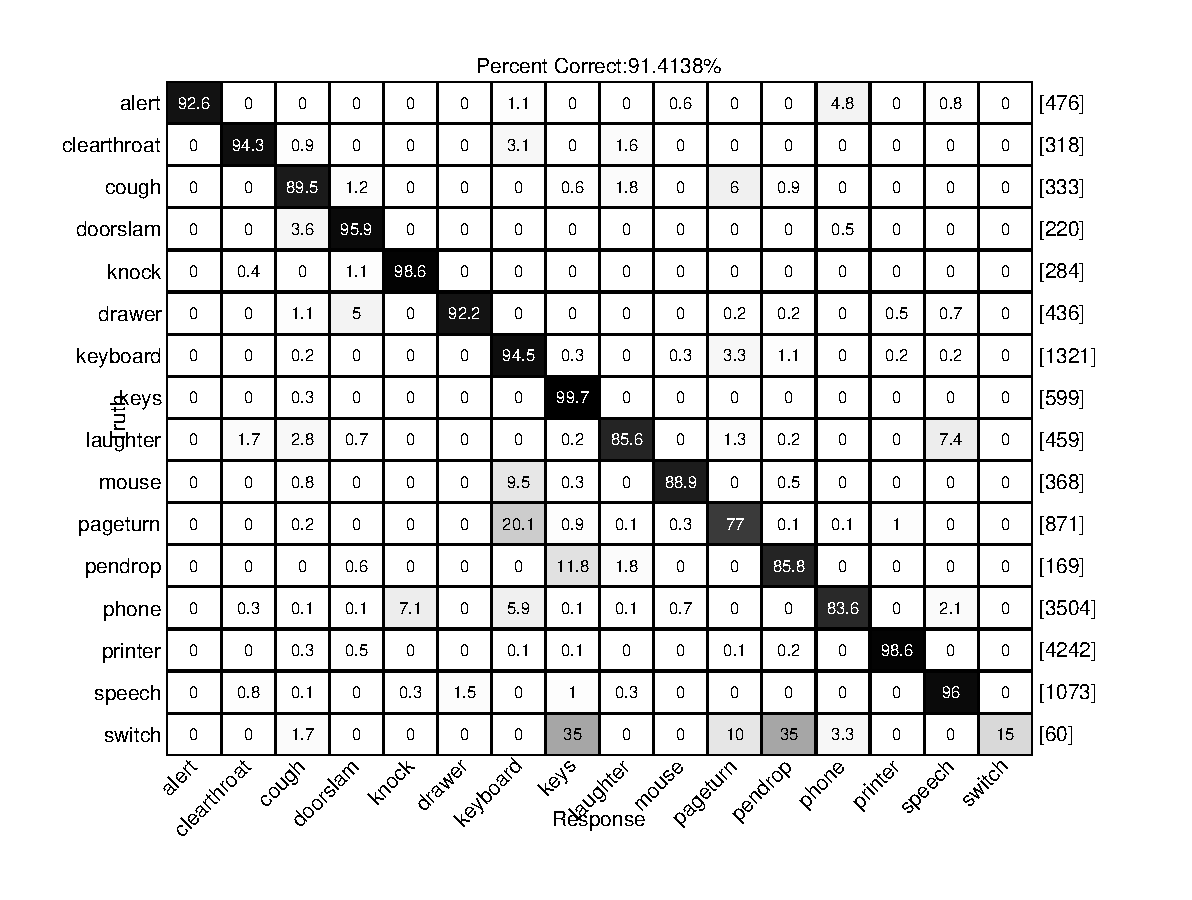
\includegraphics[width=\columnwidth]{kfolds}}
  \caption{Classifier Confusion Matrix with 5-Fold Validation}
  \label{fig:kfolds}
\end{figure}

\begin{figure}[h]
  \centering           \centerline{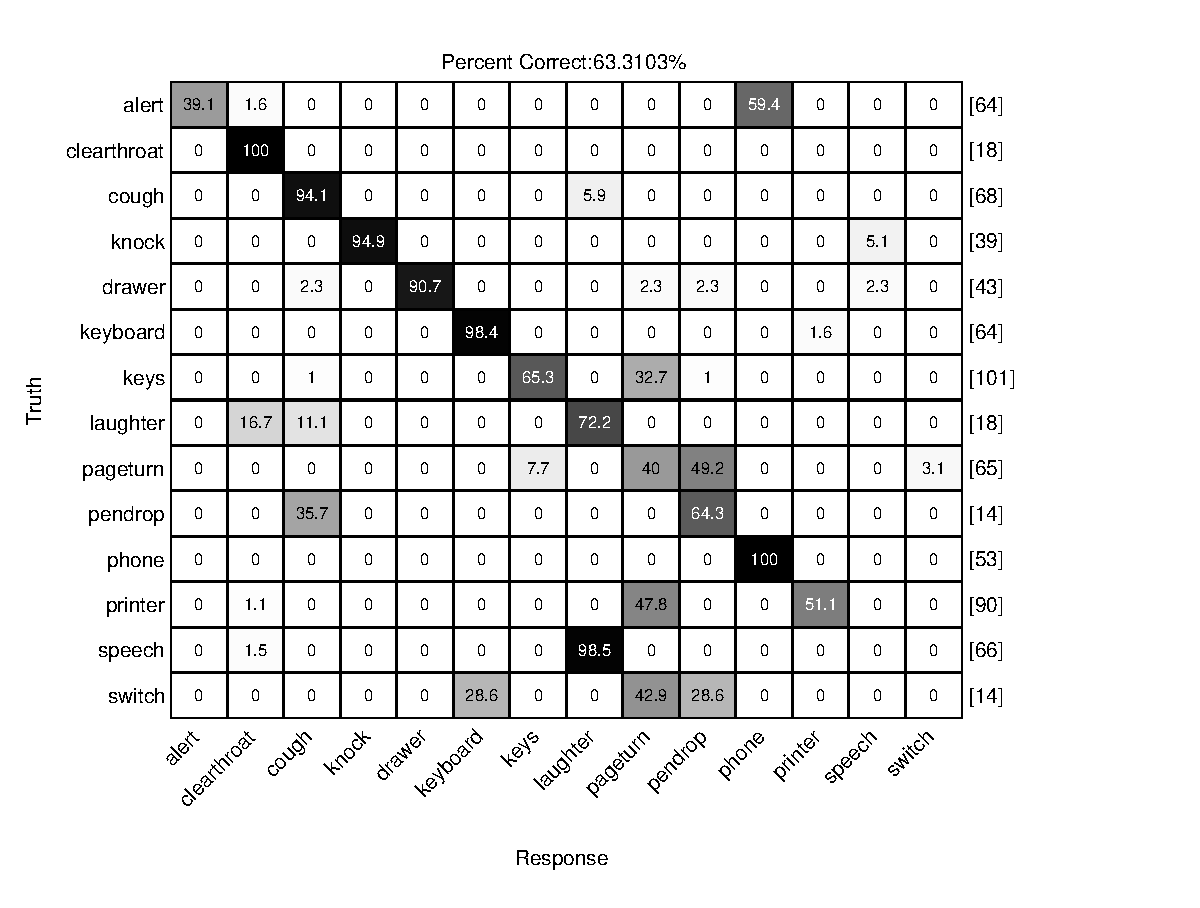
\includegraphics[width=\columnwidth]{confmatrix1}}
  \caption{Classifier Confusion Matrix with ``Perfect'' Segmentation}
  \label{fig:confmat_perfect}
\end{figure}

\begin{figure}[h]
  \centering  \centerline{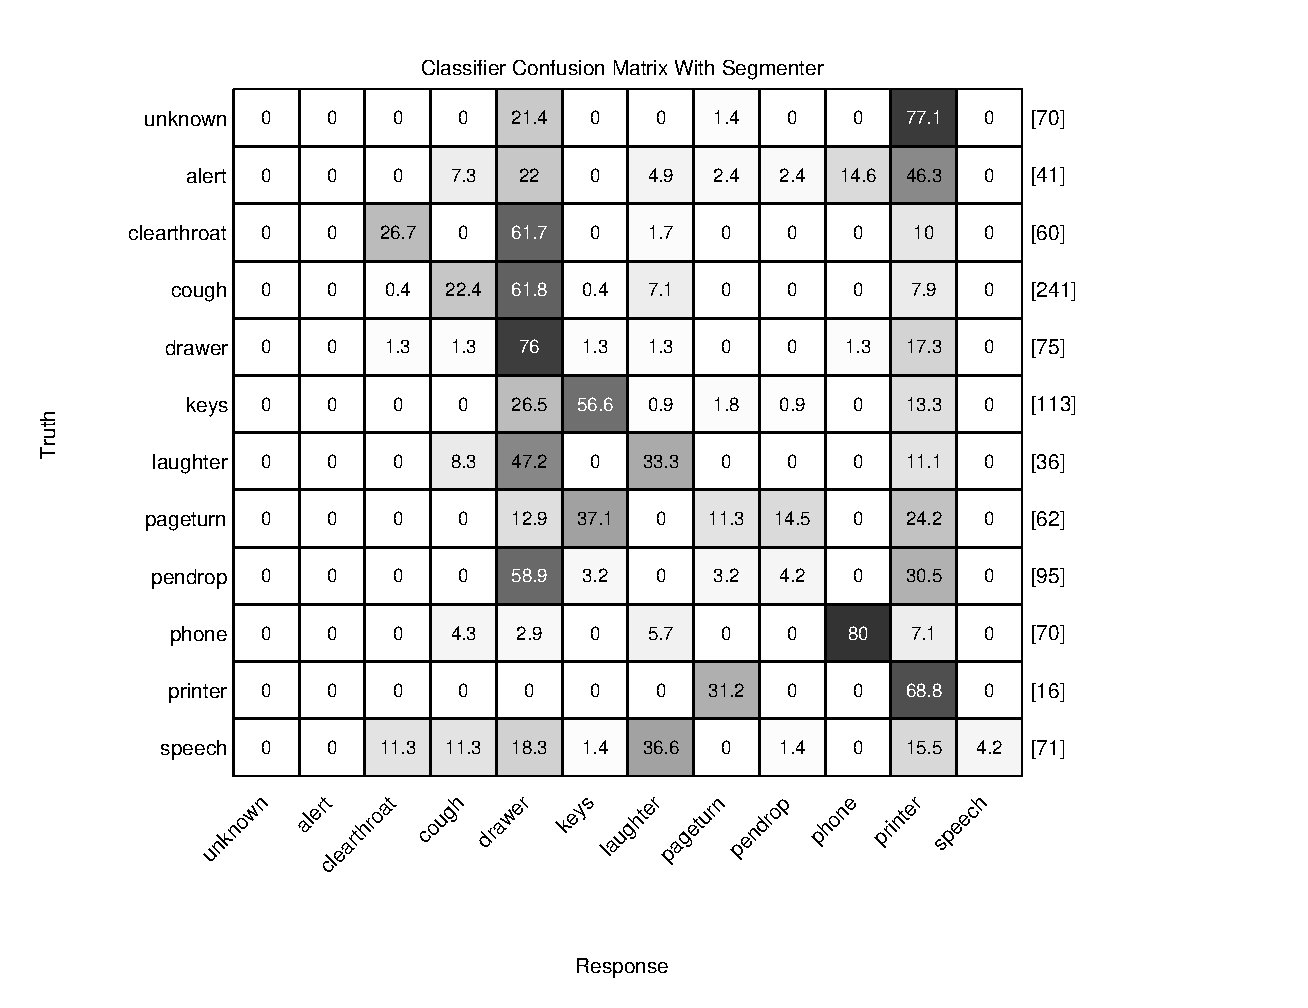
\includegraphics[width=\columnwidth]{confmatrix2}}
  \caption{Classifier Confusion Matrix with Segmenter}
  \label{fig:confmat_seg}
\end{figure}

It is worth noting that the above only hold for frame based classification. Our system was
not able to classify events as well as frames. The class of an event was chosen by taking 
the class chosen most often in the set of frames that formed the event. Because our system
is not able to accurately classify more than 50\% of frames with our segmentation this method
of classifying events does not perform well.  


\section{Conclusion}
\label{sec:conclusion}
In a k-folds sense, our classification system performed well. This implies that our system
is not deficient in features that accurately classify events in this challenge. 

The major challenges that hindered the performance of our classification were noise in the 
development set and the problem of segmenting the input file into individual events. The 
noise also posed a major challenge in segmenting the file.



% Below is an example of how to insert images. 
% -------------------------------------------------------------------------

\section{REFERENCES}
\label{sec:ref}

List and number all bibliographical references at the end 
of the paper. The references should be numbered in order 
of appearance in the document. When referring to them in 
the text, type the corresponding reference number in 
square brackets as shown at the end of this sentence 
\cite{cJones2003}, \cite{aSmith2000}. For \LaTeX\ users, 
the use of the Bib\TeX\ style file IEEEtran.bst is 
recommended, which is included in the \LaTeX\ paper 
kit available from the workshop website \cite{aaspweb}.

\section{ACKNOWLEDGMENT}
\label{sec:ack}

<<<<<<< HEAD
Available Citations:
\cite{segmentFeature}  And \cite{silenceRemove} and \cite{prt2011} and \cite{discrimPRT} and \cite{dnn}
=======
We would like to thank to Professor Sam Keene for his support and guidance. 
We would also like to thank New Folder Consulting for allowing us to use PRT.
>>>>>>> 0280de44e56d016b8f655b1d0bb0258d791aad2e

% -------------------------------------------------------------------------
% Either list references using the bibliography style file IEEEtran.bst
%\bibliographystyle{IEEEtran}
%\bibliography{refsaasp}

% or list them by yourself
 \begin{thebibliography}{5}
\bibitem{silenceRemove}
	Theodoros Giannakopoulos, ``A method for silence removal and segmentation of speech signals, implemented in Matlab",\emph{ Department of Informatics and Telecommunications University of Athens, Greece|}, 2009. Software available at \url{http://goo.gl/G3iUJ}.

\bibitem{prt2011}
 Peter Torrione and Sam Keene and Kenneth Morton, ``{PRT}: The Pattern Recognition Toolbox for {MATLAB}", 2011. Software available at \url{http://newfolderconsulting.com/prt}.

\bibitem{segmentFeature}
 	Gordern Wichern, Jiachen Xue, Harvey Thornburg, Brandon Mechtley, and Andrewwas Spanias, ``Segmentation, Indexing, and Retrieval for Environmental and Natural Sounds" in \emph{"IEEE Trans. Signal Processing}, vol. 18, pp 688--707, March 2010.

 \bibitem{dnn}
Geoffrey Hinton and Li Deng and Dong Yu and George Dahl and Abdel-rahman Mohamed and Navdeep Jaitly and Vincent Vanhoucke and Patrick Nguyen and Tara Sainath and Brian Kingsbury,  ``Deep Neural Networks for Acoustic Modeling in Speech Recognition,'' in \emph{IEEE Signal Processing Magazine}, pp. 82--97, Nov. 2012
 
 \bibitem{discrimPRT}
Xiaodong and Wu Chou. ``Discriminative Learning in Sequential Pattern Recognition,''  in \emph{IEEE Signal Processing Magazine}, pp. 14--36, Sept. 2008.
 
 \end{thebibliography}


\end{sloppy}
\end{document}
